\documentclass[tikz,12pt,margin=0px]{article}

\usepackage[a4paper, margin=1in]{geometry}
\usepackage[export]{adjustbox}
\usepackage[hungarian]{babel}
\usepackage[normalem]{ulem}
\usepackage[table,xcdraw]{xcolor}
\usepackage[thinlines]{easytable}
\usepackage[utf8]{inputenc}
\usepackage{amsmath}
\usepackage{amssymb}
\usepackage{amsthm}
\usepackage{bigints}
\usepackage{enumitem}
\usepackage{fancyhdr}
\usepackage{float}
\usepackage{fontawesome}
\usepackage{titlesec}
\usepackage{geometry}
\usepackage{graphicx}
\usepackage{hhline}
\usepackage{ifthen}
\usepackage{listings}
\usepackage{tikz}
\usepackage{makecell}
\usepackage{multirow}
\usepackage{newunicodechar}
\usepackage{pgf,tikz}
\usepackage{pgfplots}
\usepackage{pgfplotstable}
\usepackage{subcaption}
\usepackage{tikz}
\usepackage{tipa}
\usepackage{wasysym}
\usepackage{xcolor}
\usetikzlibrary{positioning,calc,shapes.multipart,arrows,arrows.meta,matrix,automata,shapes.misc,patterns}

\newcommand\ddfrac[2]{\frac{\displaystyle #1}{\displaystyle #2}}

 \geometry{
 a4paper,
 total={170mm,257mm},
 left=20mm,
 right=20mm,
 top=20mm,
 bottom=20mm
 }

\setlist[itemize,1]{label=$\bullet$}
\setlist[itemize,2]{label=$\circ$}
\setlist[itemize,3]{label=$\centerdot$}
\setlist[itemize,4]{label=$\cdot$}

\titleformat*{\section}{\Large\bfseries}
\titleformat*{\subsection}{\large\bfseries}
\titleformat*{\subsubsection}{\normalsize\bfseries}
\titleformat*{\paragraph}{\small\bfseries}
\titleformat*{\subparagraph}{\footnotesize\bfseries}

\newcommand\lword[1]{\leavevmode\nobreak\hskip0pt plus\linewidth\penalty50\hskip0pt plus-\linewidth\nobreak #1}
\pgfmathdeclarefunction{gauss}{2}{\pgfmathparse{1/(#2*sqrt(2*pi))*exp(-((x-#1)^2)/(2*#2^2))}%
}
\pagestyle{fancy}

\newcommand\blfootnote[1]{%
  \begingroup
  \renewcommand\thefootnote{}\footnote{#1}%
  \addtocounter{footnote}{-1}%
  \endgroup
}

\renewcommand{\figurename}{ábra}
\newenvironment{tetel}[1]{\paragraph{#1 \\}}{}

\newcommand{\N}{\mathbb{N}}
\newcommand{\Z}{\mathbb{Z}}
\newcommand{\R}{\mathbb{R}}
\newcommand{\Q}{\mathbb{Q}}
\newcommand{\C}{\mathbb{C}}

\makeatletter
\renewcommand\paragraph{%
	\@startsection{paragraph}{4}{0mm}%
	{-\baselineskip}%
	{.5\baselineskip}%
	{\normalfont\normalsize\bfseries}}
\makeatother

\useunder{\uline}{\ul}{}
\fancyhead{}
\cfoot{5. tétel | \thepage. oldal}

\renewcommand{\headrulewidth}{0pt}
\renewcommand{\footrulewidth}{0.4pt}

\begin{document}
    \thispagestyle{fancy}
    \hyphenation{oddword}
    \uchyph=0

    \begin{center}
        {\Large\bfseries\noindent 5. Valószínűségszámítási és statisztikai alapok} \\
    \end{center}

    \section*{Alapfogalmak}

    \noindent \textbf{Véletlen kísérlet}: Egy olyan történés / jelenség, aminek az eredményeinek halmazát ismerjük előre, de a pontos kimenet ezek között véletlen alakul. Azonos feltételek mellett megismételhető.\\

    {\small
    \noindent A kockadobásunk esetén maga a dobás a kísérlet, az eredmények halmaza {1, 2, 3, 4, 5, 6}. \\
    A (0, 1)-beli véletlen szám választása esetén az eredmények halmaza a (0, 1) intervallum.\\
    }

    \noindent \textbf{Esemény}: Egy olyan állítás, aminek az igazságtartalma a kísérlet elvégzése után kiértékelhető. Az eseményeket nagybetűvel jelöljük. Két esemény kizáró, ha egyszerre nem következhet be mindkettő. \\

    \noindent Egy A esemény \textbf{\emph{része}} egy B eseménynek (A maga után vonja B-t), ha A teljesülése esetén B mindenképp teljesül. Jelölése: $A \subseteq B$. Két esemény ekvivalens, ha mindkettő része a másiknak. Jelölése: $A = B$.
    A biztos esemény jele: $\Omega$, a lehetetlené $\varnothing$.\\

    {\small
    \noindent Kockadobás esetén az alábbiak mind események:\\
    A = \{4-et dobunk\}, B = \{4-et vagy 6-ot dobunk\}, C = \{Összetett számot dobunk\},\\
    D = \{Páratlant dobunk\}, E = \{100-nál kisebbet dobunk\}, F = \{3, 5-öt dobunk\}.\\
    A és D \emph{kizáróak}, A \emph{része} B-nek, B és C ekvivalensek, E a \emph{biztos esemény}, F pedig a \emph{lehetetlen}.\\
    }

    \noindent \textbf{Teljes eseményrendszer}: $A_1, A_2, ..., A_n, ...$ páronként kizáró események rendszere teljes \lword{eseményrendszer}, ha a kísérlet bármely kimenetele esetén valamelyik $A_i$ bekövetkezik (az alább definiált összeadást felhasználva átfogalmazható: az összegük $\Omega$).\\

    {\small
    \noindent A kockadobás esetén például\\
    T1 = \{\{párosat dobunk\}, \{páratlant pobunk\}\}, vagy\\
    T2 = \{\{1-et dobunk\}, \{prímet dobunk\}, \{4-et vagy 6-ot dobunk\}\}\\
    is \emph{teljes eseményrendszert alkot}nak.
    }

    \paragraph*{Műveletek eseményekkel\\}

    \noindent Egy A esemény \textbf{\emph{ellentettjén}} (vagy \textbf{\emph{komplementerén}}) azt az eseményt értjük, ami pontosan akkor következik be, amikor A nem. Jele $\overline{A}$.  (Pl: $\overline{\Omega} = \varnothing$).\\

    \noindent Két esemény összege (vagy uniója) az az esemény, ami pontosan akkor következik be, ha a két esemény közül legalább egy teljesül. Jele $A + B$ vagy $A \cup B$.\\

    \noindent Két esemény szorzatán (vagy metszetén) azt az eseményt értjük, ami pontosan akkor következik be, amikor mindkét esemény teljesül. Jele $A \cdot B$, $AB$ vagy $A \cap B$.

    \noindent Egy A és egy B esemény különbségén azt az eseményt értjük, amikor az A bekövetkezik, de a B nem. Jele $A  -B$ vagy $A \backslash B$.
    Valamint $A - B = A \cdot \overline{B}$.\\
\newpage
    \paragraph*{$\sigma$ algebra}

    \noindent Legyen X egy halmaz. Egy $\mathcal{R} \subseteq 2^{X}$ halmaz pontosan akkor $\boldsymbol{\sigma}$ \textbf{\emph{algebra}} X \emph{felett}, ha teljesíti az alábbi három feltételt:
    \begin{itemize}
        \item $X \in \mathcal{R}$
        \item $\mathcal{R}$ zárt a komplementerképzésre: $A \in \mathcal{R} \Rightarrow \overline{A} = X - A \in \mathcal{R}$
        \item $\mathcal{R}$ zárt a megszámlálható összegre: $A_1, A_2, \ldots, A_n, \ldots \in \mathcal{R} \Rightarrow  \sum\limits_{i}A_i \in \mathcal{R}$
    \end{itemize}

    \noindent Egy kísérlet kimeneteleinek a halmazának nem feltétlen minden eleme érdekes számunkra. A vizsgálatainkhoz fontos a kísérleten definiálható események közül a számunkra megfigyelhetőeket mindig megadni előre.\\

    \noindent \textbf{Elemi esemény}: Azokat a nem lehetetlen, megfigyelhető eseményeket, amiknek nincs olyan nem lehetetlen, megfigyelhető részeseménye, ami nem ekvivalens vele, elemi eseményeknek nevezzük. Azaz $A \in \mathcal{R}$ pontosan akkor \textbf{\emph{elemi esemény}}, ha:\\
    \[
        A \neq \varnothing\ \text{és}\ \forall B \neq \varnothing,\ B \in \mathcal{R},\ B \subseteq A : A \subseteq B
    \]
    Az elemi eseményeket $\omega$-val jelöljük.\\

    \noindent A kockadobásnál a megfelelő elemi események a következők:\\
    $\omega_1$ = \{1-et dobunk\},\ $\omega_2$ = \{2-t dobunk\},\ $\omega_3$ = \{3-mat dobunk\},\ $\omega_4$ = \{4-et dobunk\},\\
    $\omega_5$ = \{5-öt dobunk\},\ $\omega_6$ = \{6-ot dobunk\}.\\
    Lehetne elemi esemény az, hogy ”x lett a dobott érték, amit y oldalról átfordulva értünk el”, de persze ez nem célszerű választás.\\

    \noindent \textbf{Eseménytér}: Az elemi események halmaza. Mivel az összes elemi esemény összege $\Omega$, ezért az eseményteret is szokásosan $\Omega$-val jelöljük. Fontos megjegyezni, hogy abban az esetben, ha $\Omega$ nem megszámlálható, akkor az eseménytér önmagában nem határozza meg a megfigyelhető események halmazát.\\

    \noindent A kockadobás esetén az előző példában látott elemi események mellett az eseménytér
    \[\Omega = \{\omega_1,\ \omega_2,\ \omega_3,\ \omega_4,\ \omega_5,\ \omega_6\}\]

	\section*{Valószínűség}

    \noindent \textbf{Definíció}. Megfigyelhető események egy $\mathcal{R}\ \sigma$ algebráján definiálhatjuk a \textbf{\emph{valószínűség}}et, mint a következő tulajdonságokat teljesítő $P: \mathcal{R} \to [0,1]$ valós függvény:
    \begin{itemize}
      \item A valószínűség nem negatív: $0 \leq P(A)$
      \item A biztos esemény valószínűsége 1: $P(\Omega) = 1$
      \item $\forall A \in \mathcal{R}$-ra, páronként kizáró ($A_{i} \cdot A_{j} = \emptyset, i \neq j$)
      \item Kizáró események megszámlálható összegének valószínűsége a valószínűségek összege:
      \[
        A_1, A_2, \ldots, A_n, \ldots \in \mathcal{R},\ \forall i \neq j: A_iA_j = \varnothing \Rightarrow P(\bigcup\limits_{i}A_i) = \sum\limits_{i}P(A_i).
      \]
    \end{itemize}

    \noindent \textbf{Definíció}. Az eseménytér, a megfigyelhető események halmaza és a rajtuk definiált valószínűség együtt úgynevezett (\emph{\textbf{Kolmogorov-féle}}) valószínűségi mezőt alkot: $(\Omega, \mathcal{R}, P)$ hármas.\\

    {\footnotesize
    \noindent A kockadobás esetén, ha szabályos kockáról beszélünk (és minden értékű kimenetel megfigyelhető), akkor vehetjük $\ddfrac{1}{6}$-nak minden lehetséges érték valószínűségét, és így rögtön megkapjuk a 3. tulajdonságból minden esemény valószínűségét (az eseménybe foglalt lehetséges kimenetelek száma szorozva $\ddfrac{1}{6}$-al). Ha az eseménytér megszámlálható elemszámú, akkor működik is ez a módszer, azaz az elemi események valószínűségeiből minden esemény valószínűségét megkaphatjuk (nem megszámlálható esetben nem működik, például az egységintervallumon egyenletesen választott pont esetén minden egyes pont valószínűsége nulla, az intervallumok azonban már a hosszuknak megfelelő valószínűséget képviselnek).
    }
	
	\section*{Diszkrét és folytonos valószínűségi változók}
	
    \noindent \textbf{\emph{Valószínűségi változónak}} nevezünk egy eseménytér (kísérlet) elemeihez valós számokat\\
    rendelő $X : \Omega \to \mathbb{R}$ függvényt, ha
    \[
        \forall x \in \mathbb{R}: \Big\{\omega \in \Omega : X(\omega) < x\Big\} \in \mathcal{R}\ \textit{(halmaz eseményt alkot)}
    \]
	
    \noindent A kockadobás esetén legegyszerűbb módon úgy definiálhatunk egy $X$ valószínűségi változót, hogy az értékének a dobás kimenetelét adjuk.\\

    \noindent A $X$ valószínűségi változó \textbf{\emph{diszkrét}}, ha az értékkészlete véges vagy megszámlálhatóan végtelen.\\

    \noindent Ha a $X$ diszkrét valószínűségi változó értékkészlete $\left\{x_1, x_2, \ldots\right\}$, akkor a $P(X = x_i)$ számokat $X$ \textbf{\emph{eloszlás}ának} nevezzük.\\

    \noindent \textit{Megjegyzés}: Véges vagy végtelen sok szám, akkor és csak akkor alkot diszkrét eloszlást, ha nem negatívak és az összegük \textbf{1}.\\
    
    \noindent A $X$ valószínűségi változó \textbf{eloszlásfüggvénye}: $F_{X}: \mathbb{R} \to \mathbb{R}$
    \[
        F_{X}(x)= P(X < x)
    \]

    \noindent \textbf{Tétel.} Az $F_{X}: \mathbb{R} \to \mathbb{R}$ függvény pontosan akkor \textbf{\emph{eloszlásfüggvénye}} valamely valószínűségi változónak, ha
	\begin{enumerate}
		\item monoton növekvő: $\forall x_1 < x_2: F_{X}(x_1) \leq F_{X}(x_2)$
		\item balról folytonos: $\forall x_0 \in \mathbb{R}: \lim\limits_{x \to x_0^{-}}F_{X}(x) = F_{X}(x_0)$
		\item $\lim\limits_{x \to -\infty}{F_{X}(x)} = 0$
        \item $\lim\limits_{x \to +\infty}{F_{X}(x)} = 1$
	\end{enumerate}

    \noindent Egy diszkrét valószínűségi változó eloszlásfüggvénye olyan lépcsős függvény, amely a lehetséges értékeknél ugrik, és az ugrás nagysága az adott érték valószínűsége.\\
    
    \noindent Ketten lőnek céltáblára. Az $A$ találati esélye 0,7. és a $B$ találati esélye 0,8.\\
    Mindketten egy lövést adnak le egymástól függetlenül.\\
    Jelentse $X$ a találatok számát és adjuk meg az eloszlásfüggvényt!

    \begin{center}
    $\begin{array}{|c|c|}
        \hline
        \textbf{találatok száma} & \textbf{valószínűség} \\ \hline
        0 & (1-0.7) * (1-0.8) = 0.3 * 0.2 = \textbf{0.06} \\ \hline
        1 & 0.7 * (1 - 0.8) + (1-0.7) * 0.8 = 0.7*0.2 + 0.3*0.8 = \textbf{0.38}  \\ \hline
        2 & 0.7 * 0.8 = \textbf{0.56} \\ \hline
      \end{array}$\\
    \end{center}

      \begin{center}
          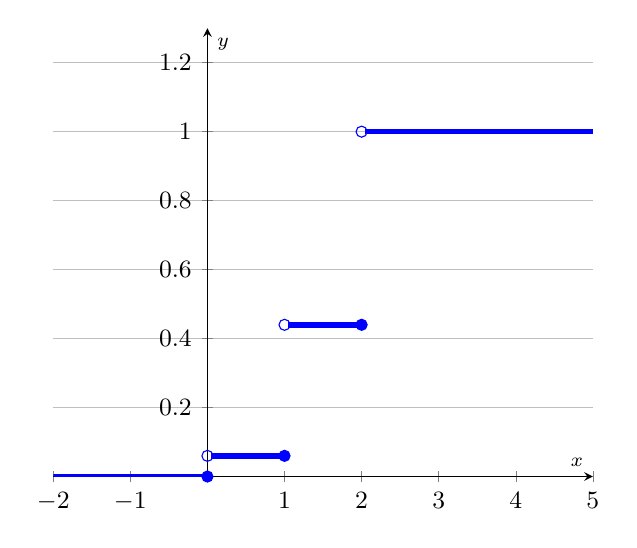
\begin{tikzpicture}[scale=1.0]
              \begin{axis}[axis lines=middle,xmin=-2.0,xmax=5.0,ymin=0.0,ymax=1.3,legend pos=north west,ymajorgrids=true,
                xlabel=$\scriptstyle x$,
                ylabel=$\scriptstyle y$,
                tick label style={font=\small}]
                \addplot[only marks,mark=*,blue] coordinates { (1.0,0.06) };
                \addplot[only marks,mark=o,blue] coordinates { (0.0,0.06) };
                \addplot[no marks,domain=0.05:1,samples=10,smooth,line width=2pt,blue]{0.06};
                \addplot[only marks,mark=*,blue] coordinates { (0,0) };
                \addplot[only marks,mark=o,blue] coordinates { (1.0,0.44) };
                \addplot[no marks,domain=1.05:2,samples=10,smooth,line width=2pt,blue]{0.44};
                \addplot[only marks,mark=*,blue] coordinates { (2,0.44) };
                \addplot[no marks,domain=-2.0:-0.05,samples=10,smooth,line width=2pt,blue]{0};
                \addplot[only marks,mark=o,blue] coordinates { (2,1) };
                \addplot[no marks,domain=2.05:5.0,samples=10,smooth,line width=2pt,blue]{1};
              \end{axis}
            \end{tikzpicture}
        \end{center}

    \noindent Ha $X$ diszkrét valószínűségi változó értékkészlete $\{x_1, x_2, \ldots\}$, akkor
    \[
        F_{X}(x) = \sum\limits_{i: x_i < x}P(X = x_i)
    \]
    
    \noindent A szabályos kockadobás esetén az előző példában definiált $X$ valószínűségi változónak adjuk meg az eloszlásfüggvényét.
    Látható, hogy az 1, 2, 3, 4, 5 és 6 értékeknél lesz csak változás, ezeken a pontokon kívül nem.\\
    Az egyes intervallumokra a megfelelő valószínűségeket kiszámolva megkapjuk, hogy
    \begin{itemize}
        \item $F_{X}(x) = 0,\ \text{ha}\ x \leq 1$,
        \item $F_{X}(x) = \ddfrac{i}{6},\ \text{ha}\ i < x \leq i + 1\ \text{és}\ 1 < x \leq 6$,
        \item $F_{X}(x) = 1,\ \text{ha}\ x > 6$.
    \end{itemize}

    \begin{figure}[H]
        \centering
        \includegraphics[width=0.39\linewidth]{img/kockadobas_eloszlasfuggveny.png}
        \caption{}
        \label{fig:imder}
    \end{figure}
    
    \noindent Legyen a $X$ diszkrét valószínűségi változó értékkészlete $\{x_1, x_2, \ldots\}$.\\
    Ekkor $X$ \emph{\textbf{várható értéke}}
    \[
        E(X) = \sum\limits_{k}x_k \cdot P(X = x_k)
    \]
    (feltéve, hogy ez a sor abszolút konvergens, azaz $\sum\limits_{k}\big|x_k\big| \cdot P(X = x_k) < \infty$).\\

    \noindent \emph{Példa}:
    \noindent 3 darab 10 dollárossal befektetési terveink vannak, egy rulett segítségével. \\
    A terv a következő: felteszünk 10 dollárt a pirosra.\\

    \noindent Ha nyer, akkor megdupláztuk a 10 dollárt és abbahagyjuk a játékot.\\
    \noindent Ha veszít, akkor újabb 10 dollárt teszünk a pirosra, és ha ezúttal nyerünk, akkor szintén abbahagyjuk a játékot.\\
    \noindent Ha másodszorra sem nyerünk, akkor az utolsó 10 dollárt is felrakjuk a pirosra.\\

    \noindent A kérdés, hogy várhatóan mennyi pénzünk lesz a tranzakció végén.\\

    \noindent A ruletten 18 piros, 18 fekete és egy zöld mező található.\\
    \noindent NY: Nyert, V: Veszített.

    \begin{center}
    \renewcommand{\arraystretch}{2}
    $\begin{array}{|ccc|c|c|}
        \hline
        1. & 2. & 3. & X_i & P(X_i) \\ \hline
        NY &  &  & 40 & \ddfrac{18}{37} = 00487 \\ \hline
        V & NY &  & 30 & \ddfrac{19}{37} \cdot \ddfrac{18}{37} = 0.25 \\ \hline
        V & V & NY & 20 & \ddfrac{19}{37} \cdot\ddfrac{19}{37} \cdot\ddfrac{18}{37} = 0.128 \\ \hline
        V & V & V & 0 & \ddfrac{19}{37} \cdot\ddfrac{19}{37} \cdot\ddfrac{19}{37} = 0.135 \\ \hline
    \end{array}$
    \renewcommand{\arraystretch}{1}
    \end{center}
    \[
        EX = \sum\limits_{k}x_k \cdot P(X = x_k) = 40 * 0,487 + 30 * 0.25 + 20 * 0.128 = 29,54
    \]
	
	\subsection*{Folytonos valószínűségi változók}
	
    \noindent A $X$ valószínűségi változó abszolút folytonos, ha létezik olyan $f_{X}: \mathbb{R} \to \mathbb{R}$ függvény, hogy $F_{X} = \bigintsss\limits_{-\infty}^{x}f_{X}(t)\ dt$ minden $x \in \mathbb{R}$ esetén. Ekkor az $f_{X}$ függvényt a $X$ valószínűségi változó \textbf{\emph{sűrűségfüggvényének}} nevezzük.\\

    \noindent \textbf{Tétel.} Egy $f:\mathbb{R} \to \mathbb{R}$ függvény, ,,akkor és csak akkor" \emph{sűrűségfüggvény}e valamilyen abszolút folytonos valószínűségi változónak, ha
    \begin{itemize}
        \item $f$ nem negatív (azaz $f(x) \geq 0,\ \forall x \in \mathbb{R}$)
        \item $\bigintss\limits_{-\infty}^{\infty}f(x)\ dx = 1$
    \end{itemize}

    \noindent \emph{Megjegyzés}:
    \begin{itemize}
        \item $P(a \leq X \leq b) = \bigintss\limits_{a}^{b}f_{X}(x)\ dx \qquad$ ($a,b \in \mathbb{R},\ a < b$ esetén)
        \item Ha $X$ abszolút folytonos valószínűségi változó, akkor $F_{X}(x)$ mindig folytonos függvény, és $f_{X}(x)$ folytonos az $x \in \mathbb{R}$ pontban, akkor $F_{X}$ differenciálható $x$-ben és $F_{X}'(x) = f_{X}(x)$.
    \end{itemize}

    \begin{center}
        \begin{tikzpicture}
            \begin{axis}[
                no markers, 
                domain=0:10, 
                samples=100,
                axis lines*=left,
                xlabel=, 
                ylabel=,
                height=6cm, 
                width=10cm,
                xtick={-3, -2, -1, 0, 1, 2, 3},
                xticklabels={, a, , , b, , }, 
                ytick=\empty,
                enlargelimits=false, 
                clip=false, 
                axis on top,
                ]
                \addplot [fill=cyan!30, draw=blue, line width=2pt, domain=-3:3] {gauss(0,1)} \closedcycle;
                \addplot [fill=orange!30, draw=orange, line width=2pt, domain=-3:-2] {gauss(0,1)} \closedcycle;
                \addplot [fill=red!30, draw=red, line width=2pt, domain=1:3] {gauss(0,1)} \closedcycle;
                \node[coordinate, pin={$P(a < X < b) = \int\limits_{a}^{b} f(x) dx$}] at (axis cs: 0, 0.4){};
                \node[coordinate, pin={$\makecell{P(b < X) =\\ \int\limits_{b}^{\infty} f(x) dx}$}] at (axis cs: 2.2, 0.0665){};
                \node[coordinate, pin={$\makecell{P(X < a) =\\ \int\limits_{-\infty}^{a} f(x) dx}$}] at (axis cs: -2.15, 0.05){};
            \end{axis}        
        \end{tikzpicture}
    \end{center}

    \begin{center} 
        $\int\limits_{-\infty}^{\infty} f_{X}(x) dx = \int\limits_{-\infty}^{a} f(x) dx + \int\limits_{a}^{b} f(x) dx + \int\limits_{b}^{\infty} f(x) dx = 1$\\
    \end{center}

    \noindent Legyen a $X$ abszolút folytonos valószínűségi változó sűrűségfüggvénye $f_{X}(x)$.\\
    Ekkor $X$ \emph{\textbf{várható értéke}}
    \[
        EX = \bigintssss\limits_{-\infty}^{\infty}x \cdot f_{X}(x)\ dx
    \]
    (feltéve, hogy ez az integrál abszolút konvergens, azaz $\bigintss\limits_{-\infty}^{\infty}\big|x\big| \cdot f_{X}(x)\ dx < \infty$)

    \noindent A $X$ valószínűségi változó \textbf{\emph{szórásnégyzete}} (vairanciája):
    \[
        D^{2}X = E\big(X - EX\big)^{2} = EX^2 - E^2X
    \]
    (feltéve, hogy ez létezik.)

    \noindent \emph{Megjegyzés}: A $X$ valószínűségi változó szórása
    \[
        DX = +\sqrt{D^{2}X}
    \]

    \begin{itemize}
    \item Ha $X$ diszkrét valószínűségi változó:
    \[
        D^{2}X = \sum\limits_{k}x_{k}^{2} \cdot P(X = x_k) - \left(\sum\limits_{k}x_k \cdot P(X = x_k)\right)^2
    \]
      
    \noindent Roulettes példa: $D^{2}X = 40^2 * 0,487 + 30^2 * 0.25 + 20^2 * 0.128 = 1055.2$
      
    \item Ha $X$ abszolút folytonos valószínűségi változó:
    \[
        D^{2}X = \bigintssss\limits_{-\infty}^{\infty}x^{2} \cdot f_{X}\ dx - \left(\bigintssss\limits_{-\infty}^{\infty}x \cdot f_{X}(x)\ dx\right)
    \]
    \end{itemize}

	\subsection*{Diszkrét valószínűségi változók}
	
	\noindent Értékkészlete legfeljebb megszámlálhatóan végtelen, azaz $\{x_1, \ldots, x_n, ... \}$ elemekből áll.\\

    \noindent Ekkor eloszlása: $p_k := P(X = x_k)$.\\
	
	\noindent \begin{tabular}{|p{3.0cm}|p{4cm}|p{4cm}|c|c|}
		\hline \textbf{Név} & \textbf{Értelmezés} & \textbf{Eloszlás} & \textbf{$EX$} & \textbf{$D^{2}X$} \\
		\hline indikátor \newline $Ind(p)$ & Egy $p$ valószínűségű esemény bekövetkezik-e vagy sem. & $P(X=1) = p$ \newline $P(X=0) = 1-p$ & $p$ & $p(1-p)$ \\
		\hline geometriai (Pascal) \newline $Geo(p)$ & Hányadikra következik be először egy $p$ valószínűségű esemény. & \makecell{$P(X=k) =$\\ $p(1-p)^{k-1}$} \newline $k=1,2...$ & $\ddfrac{1}{p}$ & $\ddfrac{1-p}{p^2}$\\
        \hline \multicolumn{5}{l}{\makecell{Ha a kísérletünk a kockadobás az első 6-os dobásig és az\\ X valószínűségi változó a dobások száma, akkor 6 geometriai eloszlású.}} \\
		\hline hipergeometriai \newline $Hipgeo(N,M,n)$ & Visszatevés nélküli mintavétel. & $P(X=k) = \ddfrac{{M \choose k}{N-M \choose n-k}}{{N \choose n}}$ \newline $k=0,1,...,n$ & $n \ddfrac{M}{N}$ & $n \ddfrac{M}{N}(1 - \ddfrac{M}{N})(1 - \ddfrac{n-1}{N-1})$ \\
        \hline \multicolumn{5}{l}{\makecell{Ha N és M a végtelenbe tart úgy, hogy M / N egy 0 és 1 közötti p konstanshoz tart, akkor\\ a hipergeometrikus eloszlások sorozata a binomiális eloszláshoz tart.}}\\
		\hline binomiális \newline $Bin(n,p)$ & Visszatevéses mintavétel. & $P(X=k) = {n \choose k}p^{k}(1-p)^{n-k}$ \newline $k=0,1,...,n$ & $np$ & $np(1-p)$ \\
		\hline negatív binomiális \newline $Negbin(n,p)$ & Hányadikra következik be $n.$ alkalommal egy $p$ valószínűségű esemény. & $P(X=k) = {k-1 \choose n-1}p^{n}(1-p)^{k-n}$ \newline $k=n,n+1,...$ & $\ddfrac{n}{p}$ & $\ddfrac{n(1-p)}{p^{2}}$ \\
		\hline Poisson \newline $Poi(\lambda)$ & Ritka esemény. & $P(X=k) = \ddfrac{\lambda^k}{k!}e^{-\lambda}$ & $\lambda$ & $\lambda$ \\
		\hline
	\end{tabular}\\ \\

    \noindent \emph{Példa}:\\ 
    
    \noindent \textbf{\emph{Hipergeometrikus}}:\\
    
    \noindent \emph{Egy úton 30 nap alatt 12 napon történt baleset. Ebből a 30 napból kiválasztunk egy hetet, mi a valószínűsége, hogy ezen a héten 2 balesetes nap van?}\\
    
    \noindent Hipergeometriainál ismert, hogy mennyi az összes elem és az összes selejt N, K, és a minta n.\\
    \noindent Az összes elem $N = 30$ nap, ebből (selejtes) a balesetes nap, $M = 12$. A minta egy hét, vagyis $n = 7$, és itt $X = 2$ balesetes napot szeretnénk.\\

    \begin{center}
        $P(X=k) = \ddfrac{{M \choose k}{N-M \choose n-k}}{{N \choose n}} = \ddfrac{{12 \choose 2}{30-12 \choose 7-2}}{{30 \choose 7}} = \ddfrac{{12 \choose 2}{18 \choose 5}}{{30 \choose 7}} = \ddfrac{565488}{2035800} = 0.27777188$\\
        $EX = n * \ddfrac{M}{N} = 7 * \ddfrac{12}{30} = 0.23^{.}$
    \end{center}
    
    \noindent A másik két feladatban csak valamilyen százalékos érték, a várható, az átlag, az arány vagy valószínűség. Ez esetben nem tudjuk, hogy mennyi baleset történik a 30 nap alatt, csak azt tudjuk, hogy várhatóan mennyi.\\
    
    \noindent \textbf{\emph{Binomiális:}}\\
    Egy úton 30 nap alatt átlag 12 balesetes nap van. Mi a valószínűsége, hogy egy adott héten 2 balesetes nap van?\\

    \noindent A binomiálisnál vett példában nem lehet több a balesetes napok száma, mint 7, így X korlátos.\\
    $X$ = balesetes napok száma.\\
    $n = 7$, $p = \ddfrac{M}{N} = \ddfrac{12}{30} = 0.4$.\\
    
    \begin{center}
        $P(X = k = 2) = {n \choose k}p^{k}(1-p)^{n-k} = {7 \choose 2}*0.4^{2}*(1 - 0.4)^{7-2} = 21*0.16*0.07776 = 0.2612736$
        $EX = n * p = 7 * 0.4 = 2.8$
    \end{center}
    
    \noindent \textbf{\emph{Poisson:}}\\
    Egy úton 30 nap alatt átlag 12 baleset történik. Mi a valószínűsége, hogy egy adott héten 2 baleset van?\\
    Az első két esetben X a balesetes napok száma, a harmadikban pedig a balesetek száma.\\
    
    \noindent A harmadik feladatnál a Poisson eloszlás esetében baleset tetszőleges számú lehet, átlagban 12 30 naponta, de lehet akár 1000 is, tehát itt X nem korlátos.\\
    $X$ = balesetek száma.\\
    $\lambda =$ várhatóan hány baleset van egy héten 30 naponta 12 baleset szokott lenni, tehát naponta $\ddfrac{12}{30} = 0.4$ és így hetente hétszer annyi $7 * 0.4 = 2.8$.\\
    \begin{center}
        $P(X = k = 2) = \ddfrac{\lambda^k}{k!}e^{-\lambda} = \ddfrac{2.8^2}{2!}e^{-2.8} = \ddfrac{7.84}{2} * 0.0608101 = 0,238375592$\\
        $E(X) = \lambda = 2.8$\\
    \end{center}

	\noindent \begin{tabular}{|p{3cm}|c|c|c|c|}
		\hline \textbf{Név} & \textbf{Eloszlásfüggvény} & \textbf{Sűrűségfüggvény} & \textbf{$EX$} & \textbf{$D^{2}X$} \\
		\hline egyenletes \newline $E(a,b)$
		& $\left\{\begin{array} {lr}
					0 & x \leq a \\
					\ddfrac{x-a}{b-a} &  a < x \leq b \\
					1 & b < x
			\end{array}\right.$
		& $\left\{\begin{array} {lr}
					\ddfrac{1}{b-a} & a < x \leq b \\
					0 & \text{különben}
			\end{array}\right.$
		& $\ddfrac{a+b}{2}$
		& $\ddfrac{(b-a)^2}{12}$ \\
		\hline exponenciális \newline $Exp(\lambda)$
		&  $\left\{\begin{array} {lr}
					1 - e^{-\lambda x} & x \geq 0 \\
					0 &  \text{különben}
			\end{array}\right.$
		&  $\left\{\begin{array} {lr}
					\lambda \cdot e^{-\lambda x} & x \geq 0 \\
					0 & \text{különben}
			\end{array}\right.$
		& $\ddfrac{1}{\lambda}$
		& $\ddfrac{1}{\lambda^{2}}$ \\
		\hline normális \newline $N(m,\sigma^2)$ & $...$ & $\ddfrac{1}{\sqrt{2 \pi}\sigma}e^{-\ddfrac{(x-m)^2}{2\sigma^2}}$ $x \in \mathbb{R}$ & $m$ & $\sigma^2$ \\
		\hline standard normális \newline $N(0,1^2)$ & $\Phi(x)=...$ & $\ddfrac{1}{\sqrt{2 \pi}}e^{-\ddfrac{x^2}{2}}$ $x \in \mathbb{R}$ & $0$ & $1$ \\
		\hline gamma \newline $\Gamma(\alpha,\lambda)$
		& $...$
		& $\left\{\begin{array} {lr}
					\ddfrac{1}{\Gamma(\alpha)}\lambda^{\alpha}x^{\alpha-1}e^{-\lambda x} & x \geq 0 \\
					0 & \text{különben}
			\end{array}\right.$
		& $\ddfrac{\alpha}{\lambda}$
		& $\ddfrac{\alpha}{\lambda^2}$ \\
		\hline
	\end{tabular}\\

	\subsection*{Fogalmak}
	
	\begin{itemize}
		\item \textit{Konvolúció}: $X,Y$ független valószínűségi változók, konvolúciójuk az $X+Y$ v. v.
		\item \textit{Függetlenség}: $P(X_1<x_1, ..., X_n<x_n) = \prod\limits_{i=1}^{n}{P(X_i<x_i)}$ vagy diszkrét esetben:
        \[
            P(X_1)x_1, \ldots, X_n=x_n) = \prod_{i=1}^{n}{P(X_i=x_i)}
        \]
        \item \textit{Várható érték}: $(\Omega, \mathcal{R}, P)$ valószínűségi mező, $X:\Omega \to \mathbb{R}$ valószínűségi változó, $EX = \int_{\Omega}{XdP}$, ha ez létezik. Diszkrét esetben $EX = \sum_{k}{x_k \cdot p_k}$, ha abszolút konvergens. Abszolút folytonos esetben $EX = \int_{-\infty}^{\infty}{x \cdot f(x)dx}$, ha abszolút folytonos.
		\item \textit{Szórásnégyzet}: $D^{2}X = E\big((X-EX)^2\big) = EX^2-E^{2}X$
		\item \textit{$l.$ momentum}: $EX^l = \int\limits_{\Omega}{x^{l}dP}$, ha létezik.
		\item \textit{Szórás}: $DX = \sqrt{D^{2}X}$
		\item \textit{Kovariancia}: $cov(X,Y) = E((X-EX)(Y-EY) = E(XY) - EX \cdot EY$. Ha $cov(X,Y) = 0$, akkor $X$ és $Y$ korrelálatlan. (Megjegyzés: ha két v.v. független, akkor $cov(X,Y) = 0$, vagyis korrelálatlanok; illetve $cov(X,X) = D^{2}X$.)
		\item \textit{Korreláció}: $R(X,Y) = \ddfrac{cov(X,Y)}{DX \cdot DY}$, két v.v. lineáris kapcsolatát méri. 
        \begin{itemize}
            \item $R > 0 \to$ pozitív 
            \item $R < 0 \to$ negatív 
            \item $R^2 \sim 0 \to$ gyenge
            \item $R^2 \sim 0.5 \to$ közepes
            \item $R^2 \sim 1 \to$ erős
        \end{itemize}
	\end{itemize}
	
	\section*{Nagy számok törvénye}
	
	\subsection*{Gyenge törvény}
	
	$X_1, X_2, ...$ függetlenek, azonos eloszlásúak, $EX_i = m < \infty$, $D^{2}X_i = \sigma^2 < \infty$. \\
	\[
        P\left(\ddfrac{X_1 + ... + X_n}{n} - m \geq \varepsilon\right) \rightarrow 0 \quad (n \to \infty)
    \]
    $\forall \varepsilon > 0$\text{-ra (sztochasztikus konvergencia)}.

	\subsection*{Erős törvény}
	
	$X_1, X_2, ...$ függetlenek, azonos eloszlásúak, $EX_1 = m < \infty$, $D^{2}X_1 = \sigma^2 < \infty$. \\
	\[
        \ddfrac{X_1 + ... + X_n}{n} \rightarrow m \quad (n \to \infty)
    \]
    1 valószínűséggel. \\
	Megjegyzés: Csebisev-egyenlőtlenséggel bizonyítjuk. $\Big(\ddfrac{\sigma^2}{n \varepsilon^2} \to 0$ $(n \to \infty)\Big)$
	
	\subsubsection*{Csebisev-egyenlőtlenség}
	
	$EX$ véges. \\
	Ekkor $P(|X-EX| \geq \lambda) \leq \ddfrac{D^{2}X}{\lambda^2}$ \\
	Megjegyzés: Bizonyítás Markov-egyenlőtlenséggel.
	
	\subsubsection*{Markov-egyenlőtlenség}
	
	$X \geq 0, c > 0$. \\
	Ekkor $P(X \geq c) \leq \ddfrac{EX}{c}$
	
	\subsection*{Konvergenciafajták}
	
	$X_n \to X$, vagyis $X$ konvergens.
	\begin{itemize}
		\item \textit{sztochasztikusan}: ha $\forall \varepsilon > 0$-ra $P(|X_n - X| \geq \varepsilon) \rightarrow 0$ $(n \to \infty)$.
		\item \textit{1 valószínűséggel (majdnem mindenütt)}: ha $P(\omega : X_n(\omega) \to X(\omega)) = 1$.
		\item \textit{$L^p$-ben}: ha $E(|X_n - X|^p) \rightarrow 0$ $(n \to \infty)$ ($p>0$ rögzített).
		\item \textit{eloszlásban}: ha $F_{X_n}(x) \rightarrow F_{X}(x)$ $(n \to \infty)$ az utóbbi minden folytonossági pontjában.
	\end{itemize}
	\textit{Kapcsolataik}: 1 valószínűségű és $L^p$-beli a legerősebb, ezekből következik a sztochasztikus, ebből pedig az eloszlásbeli.
	
	\section*{Centrális határeloszlás tétel}
	
	$X_1, X_2, ...$ függetlenek, azonos eloszlásúak, $EX_1 = m < \infty$, $D^{2}X_1 = \sigma^2 < \infty$. \\
	Ekkor $\ddfrac{X_1 + ... + X_n - nm}{\sqrt{n}\sigma} \rightarrow N(0,1)$ $(n \to \infty)$ eloszlásban, azaz
    \[
        P\left(\ddfrac{X_1 + ... + X_n - nm}{\sqrt{n}\sigma} < x\right) \rightarrow \Phi(x)\quad (n \to \infty)
    \]
	
	\section*{Statisztikai mező}
	
	$(\Omega, \mathcal{R}, \mathcal{P})$ hármas, ha $\mathcal{P} = \{P_{\vartheta}\}_{\vartheta \in \Theta}$ és $(\Omega, \mathcal{R}, P_{\vartheta})$\\
    Kolmogorov-féle valószínűségi mező $\forall \vartheta \in \Theta$-ra.
	
	\subsection*{Fogalmak}
	
	\begin{itemize}
		\item \textit{Minta}: $\underline{X} = (X_1,...,X_n): \Omega \to X \in \mathbb{R}^n$. ($X_i$ valószínűségi változó)
		\item \textit{Mintatér}: $X$, minta lehetséges értékeinek halmaza, gyakran $\mathbb{R}^n, \mathbb{Z}^n$.
		\item \textit{Minta [realizációja]}: $\underline{x} = (x_1,...,x_n)$, konkrét megfigyelés.
		\item \textit{Statisztika}: $T: X \to \mathbb{R}^k$.
		\item \textit{Statisztika alaptétele}: (Glivenko--Cantelli-tétel) $X_1, X_2, ...$ független, azonos eloszlású $F$ eloszlásfüggvénnyel. Ekkor az $F_n$ tapasztalati eloszlásfüggvényre teljesül, hogy
        \[
            \sup_{-\infty<x<\infty}{|F_n(x) - F(x)|} \to 0 \quad (n \to \infty)
        \]
        1 valószínűséggel.
	\end{itemize}
	
	\section*{Statisztikai becslések}
	
	$(\Omega, \mathcal{R}, \mathcal{P})$ statisztikai mező, $\vartheta \in \Theta$, $P_{\vartheta}(X_1<x_1,...,X_n<x_n) = F_{\vartheta}(\underline{x})$ \\
	$T(\underline{X})$ a $\vartheta$ \textit{becslése}, ha $T: \mathbb{R}^n \to \Theta$. \\
	$T(\underline{X})$ a $h(\vartheta)$ \textit{becslése}, ha $T: \mathbb{R}^n \to h(\Theta)$. \\
	\textit{Torzítatlanság}: $T(\underline{X})$ torzítatlan becslése $h(\vartheta)$-nak, ha $E_{\vartheta}T(\underline{X}) = h(\vartheta)$ $\forall \vartheta \in \Theta$. \\
	\textit{Aszimptotikusan torzítatlan}: $T(\underline{X})$ aszimptotikusan torzítatlan a $h(\vartheta)$-ra, ha $E_{\vartheta}T(\underline{X}) \to h(\vartheta)$ $(n \to \infty)$ $\forall \vartheta \in \Theta$. \\
	A $T_1$ torzítatlan becslés \textit{hatásosabb} $T_2$ torzítatlan becslésnél, ha $D_{\vartheta}^{2}T_1 \leq D_{\vartheta}^{2}T_2$ $\forall \vartheta \in \Theta$. \\
	Hatásos, ha minden más torzítatlan becslésnél hatásosabb. Ha van hatásos becslés, akkor az egyértelmű.
	
	\begin{itemize}
		\item \textit{Maximum-likelihood becslés}: Likelihood függvény: $L(\vartheta, \underline{x}) = \left\{\begin{array} {lr}
		P_{\vartheta}(\underline{X} = \underline{x}) & diszkr. \\
		f_{\vartheta, \underline{X}}(\underline{x}) & absz. folyt.
		\end{array}\right.$ \\
		Független esetben: $L(\vartheta, \underline{x}) = \left\{\begin{array} {lr}
		\prod_{i=1}^{n}{P_{\vartheta}(X_i = x_i)} & diszkr. \\
		\prod_{i=1}^{n}{f_{\vartheta, X_i}(x_i)} & absz. folyt.
		\end{array}\right.$\\
		$\hat{\vartheta}$ a $\vartheta$ ismeretlen paraméter maximum-likelihood becslése, ha $L(\hat{\vartheta},\underline{X}) = \max_{\vartheta \in \Theta}{L(\vartheta,\underline{X})}$.
		\item \textit{Momentum-módszer becslés}: $\vartheta = (\vartheta_1, ..., \vartheta_k)$, $X_1, ..., X_n$, $l.$ momentum: $M_l(\underline{\vartheta}) = E_{\underline{\vartheta}}X_{i}^{l}$, tapasztalati $l.$ momentum: $\hat{M}_l = \ddfrac{\sum_{i=1}^{n}{X_i^l}}{n}$. \\ $\hat{\underline{\vartheta}}$ a $\underline{\vartheta}$ momentum módszer szerinti becslése, ha megoldása az $M_l(\underline{\vartheta}) = \hat{M}_l$, $l=1..k$ egyenletrendszernek.
	\end{itemize}
	
	\section*{Hipotézisvizsgálat}
	
	Felteszünk egy hipotézist, és vizsgáljuk, hogy igaz-e. Elfogadjuk vagy elutasítjuk. Lehet paraméteres vagy nem paraméteres, vizsgálhatjuk várható értékek, szórások egyezőségét, értékét, teljes eseményrendszerek függetlenségét. Illeszkedésvizsgálattal megállapíthatjuk, hogy a valószínűségi változók adott eloszlásfüggvényűek-e, homogenitásvizsgálattal pedig azt, hogy ugyanolyan eloszlású-e két minta. \\
	$H_0$: nullhipotézis, $\vartheta \in \Theta_0$; $H_1$: ellenhipotézis, $\vartheta \in \Theta_1$; $\Theta = \Theta_0 \bigcup \Theta_1$. \\
	\textit{Egy- és kétoldali vizsgálat}: Kétoldali ellenhipotézisnél a nem egyezőséget tesszük fel, egyoldalinál valamilyen relációt. Kétoldalinál a próba értékének abszolút értékét vizsgáljuk, hogy az elfogadási tartományon belül van-e, ekkor például az u-próbánál az adott hibaszázalékot meg kell felezni a számításhoz, hiszen a $\Phi$ függvény szimmetrikus az $y$ tengelyre.
	\begin{itemize}
	\item \textit{Statisztikai próba}: $X = X_e \bigcup X_k$ (diszjunkt halmazok) elfogadási és kritikus tartomány. Ez a felbontás a statisztikai próba. Ha a megfigyelés eleme a kritikus tartománynak, akkor elutasítjuk a nullhipotézist, ha nem eleme, akkor elfogadjuk. $T(\underline{x}) = \left\{\begin{array} {lr} 1 & x \in X_k \\ 0 & otherwise \end{array}\right.$
	\item \textit{Elsőfajú hiba}: $H_0$ igaz, de elutasítjuk. Valószínűsége: $P_{\vartheta}(\underline{X} \in X_k)$, $\vartheta \in \Theta_0$.
	\item \textit{Másodfajú hiba}: $H_0$ hamis, de elfogadjuk. Valószínűsége: $P_{\vartheta}(\underline{X} \notin X_k)$, $\vartheta \in \Theta_1$. \\
	Az a cél, hogy ezek a hibák minél kisebbek legyenek. Egymás kárára javítható a két valószínűség, ha a megfigyelések száma rögzített.
	\item \textit{Próba terjedelme}: $\alpha$ a próba terjedelme, ha $P_{\vartheta}(\underline{X} \in X_k) \leq \alpha$, $\vartheta \in \Theta_0$. \\
	$\alpha$ a próba pontos terjedelme, ha $\sup_{\vartheta \in \Theta_0}{P_{\vartheta}(\underline{X} \in X_k) = \alpha}$.
	\end{itemize}
	
	\section*{Klasszikus statisztikai próbák}
	
    \subsection*{Alapfogalmak\\}

    \noindent \textbf{\emph{Alaphipotézis}}nek vagy \textbf{\emph{nullhipotézis}}nek $(H_0)$ nevezzük az alapfelvetésünket, amit igazolni szeretnénk. Ezzel szemben áll az ellenhipotézis, ami akkor teljesül, ha a nullhipotézis nem igaz.\\

    \noindent \emph{\textbf{Elfogadási tartomány}}nak nevezünk egy olyan halmazt, amelyben a nullhipotézis teljesülése esetén a vizsgált statisztika értéke nagy valószínűséggel $(1-p)$ elhelyezkedik. Ezzel szemben a \textbf{\emph{kritikus tartomány}}ba várhatóan akkor esik a $h$ statisztika értéke, ha az ellenhipotézis teljesül.

    \begin{center}
        \noindent \textbf{Hibák} \qquad
      \begin{tabular}{c|cc}
         & $H_0$ igaz & $H_0$ hamis \\ \hline
        $H_0$ elfogadása & helyes döntés & másodfajú hiba \\
        $H_0$ elvetése & elsőfajú hiba & helyes döntés \\
      \end{tabular}
    \end{center}

    \noindent Egy \textbf{\emph{próba terjedelme}} az elsőfajú hiba valószínűségének felső határa.\\

    \noindent Ha $\beta$ a másodfajú hiba valószínűsége, akkor a \textbf{\emph{próba erőfüggvénye}}: $1 - \beta$.\\

    \noindent Azonos terjedelmű próbák közül \textbf{\emph{erősebb}}nek nevezzük azt, amelyiknek az erőfüggvénye minden ponton nem kisebb a másikénál.\\

    \noindent Továbbiakban:
    \begin{itemize}
        \item X normális eloszlású, ismert szórású változó $n$ elemű mintája:
        \[X_i \sim N(m, \sigma^2)),\quad i=1,\ldots,n\]
        \item X, Y egymástól független normális eloszlású, ismert szórású változó $n, m$ elemű mintája:
        \begin{center}
            $X_i \sim N(m, \sigma^2)),\quad i=1,\ldots,n$, \\
            $\eta_j \sim N(m_2, \sigma_2^2),\quad j=1,\ldots, m$
        \end{center}
        \item $\overline{X}$ a vizsgált valószínűségi változó átlaga a mintában,
        \item $m_{i}$ az előre megadott érték, amihez az átlagot viszonyítjuk,
        \item $\sigma$ a vizsgált valószínűségi változó ismert szórása.
    \end{itemize}

    \subsection*{u-próbák}

    \subsubsection*{Egymintás eset}

    \noindent A próba azt ellenőrzi, hogy egy adott statisztikai ismérv esetén a mintabeli átlag szignifikánsan eltér-e a populációs átlagtól. Más szavakkal, hogy egy valószínűségi változó átlaga szignifikánsan különbözik-e egy adott $m$ értéktől.\\

    \noindent Adott egy X normális eloszlású, ismert szórású változó $n$ elemű mintája. Nullhipotézisünk az, hogy a várható érték megegyezik-e egy konkrét értékkel ($H_0 : m = m_0$), másképpen fogalmazva azt vizsgáljuk, hogy a mintabeli átlag nem tér-e el szignifikánsan $m_0$-tól.\\

    \noindent Legyen a próbastatisztika:
    \[
        u = \sqrt{n}\ddfrac{\overline{X}- m_0}{\sigma}
    \]

    \noindent Ekkor a $p$ valószínűség mellett elfogadjuk a nullhipotézist, ha $\big|u\big| \leq u_{\frac{p}{2}}$, ahol $u_{\frac{p}{2}}$ a standard normális eloszlás $1-\frac{p}{2}$ kvantilise. Ha igaz a nullhipotézis, akkor ez közel standard normális eloszlású.\\

    \noindent Ha az ellenhipotézis egyoldalú, akkor az elfogadási tartomány $u \leq u_p$-re, illetve $u \geq -u_p$-re módosul.\\

    \subsubsection*{Kétmintás eset}

    \noindent A próba azt vizsgálja, hogy egy valószínűségi változó átlaga két külön mintában szignifikánsan különböző-e.\\

    \noindent Két független (a fenti feltételeket teljesítő) mintára $(X, Y)$ vonatkozó nullhipotézisünk, hogy várható értékük egyenlő ($H_0 : m_1 = m_2$). Erre a próbastatisztika:
    \[
        u = \ddfrac{\overline{X} - \overline{Y}}{\sqrt{\ddfrac{\sigma_{x}^{2}}{n_x} + \ddfrac{\sigma_{y}^{2}}{{n_y}}}}
    \]

    \noindent \textbf{Tétel.} Az $u$-próbák konzisztens, torzítatlan és legerősebb próbák.\\

	\begin{itemize}
		\item \textit{u-próba}: Feltételezzük, hogy a minta normális eloszlású ($X_i \sim N(m, \sigma^2)$), $i=1..n$, és hogy a szórás ismert.
			\begin{itemize}
        \item \textit{Egymintás}: A nullhipotézis az, hogy a várható érték megegyezik-e egy konkrét értékkel ($m_0$), másképpen fogalmazva azt vizsgáljuk, hogy a mintabeli átlag nem tér-e el szignifikánsan $m_0$-tól. Tehát $H_0: m = m_0$, és kétoldali esetben $H_1: m \neq m_0$, egyoldaliban pedig például $H_1: m \geq m_0$ vagy $H_1: m < m_0$. \\
				Az u-próba értéke: $u = \sqrt{n}\ddfrac{\overline{X} - m_0}{\sigma}$. Ha igaz a nullhipotézis, akkor ez közel standard normális eloszlású. \\
				$\varepsilon$ hibavalószínűséggel vizsgáljuk a hipotézist, ehhez szükségünk van a $\Phi(u_{1-\varepsilon}) = 1 - \varepsilon$ értékre. \\
				Kétoldali esetben $H_0$-t elutasítjuk, ha $|u| > u_{1-\ddfrac{\varepsilon}{2}}$, és elfogadjuk, ha $|u| \leq u_{1-\ddfrac{\varepsilon}{2}}$. \\
				Egyoldali esetben $u > u_{1-\varepsilon}$ (jobb) és $u < u_{1-\varepsilon}$ (bal) esetét vizsgáljuk, ezen esetekben utasítjuk el $H_0$-t.
		\item \textit{Kétmintás}: Itt a feltételek a következők: $X_i \sim N(m_1, \sigma_1^2)$, $i=1..n$ és $\eta_j \sim N(m_2, \sigma_2^2)$, $j=1..m$. A szórások szintén ismertek. $H_0: m_1 = m_2$, és $u = \ddfrac{\overline{X} - \overline{\eta}}{\sqrt{\ddfrac{\sigma_1^2}{n} + \ddfrac{\sigma_2^2}{m}}}$. $H_1 : m_1 > m_2$, ez a felső (jobb?) oldali, $H_1 : m_1 < m_2$ pedig az alsó (bal?) ellenhipotézis.
			\end{itemize}
		\item \textit{t-próba}:	Ennél a próbánál nem ismert a szórás, viszont ugyanúgy normális eloszlást feltételezünk, mint az u-próbánál. $X_i \sim N(m, \sigma^2)$, $i=1..n$.
			\begin{itemize}
				\item \textit{Egymintás}: $H_0: m = m_0$. Ellenhipotézis az u-próbához hasonlóan. $t = \sqrt{n}\ddfrac{\overline{X} - m_0}{\sqrt{\sigma_{*}^2}}$, ahol $\sigma_{*}^2$ a korrigált tapasztalati szórásnégyzet, amit a mintából számíthatunk ki. (Megjegyzés: $n$ helyett $n-1$-gyel osztunk a képletben.) Ez az érték $t$-eloszlású $H_0$ esetén, ami $n-1$ szabadságfokú. Más néven szokás ezt a próbát Student-próbának is nevezni.
				\item \textit{Kétmintás}: $X_i \sim N(m_1, \sigma_1^2)$, $i=1..n$ és $\eta_j \sim N(m_2, \sigma_2^2)$, $j=1..m$. Ez esetben sem ismert a szórás, viszont feltételezzük, hogy a két minta szórása megegyezik. Ekkor $t_{n+m-2} = \sqrt{\ddfrac{nm(n+m-2)}{n+m}}\ddfrac{\overline{X} - \overline{\eta}}{\sqrt{\sum{(X_i - \overline{X})^2} + \sum{(\eta_j - \overline{\eta})^2}}}$. $n+m-2$ a próba szabadságfoka.
			\end{itemize}
		\item \textit{f-próba}: Két minta esetén használható. Ez a próba szórások egyezőségének vizsgálatára alkalmas, tehát itt $H_0 : \sigma_1 = \sigma_2$. Ha a két minta szórásnégyzete megegyezik, akkor a hányadosuk $1$-hez tart. $f_{n-1,m-1} = max(\ddfrac{\sigma_1^2}{\sigma_2^2}, \ddfrac{\sigma_2^2}{\sigma_1^2})$. A két szabadsági fok közül az első az $f$ számlálójához tartozó minta elemszáma $- 1$, a második a nevezőjéhez.
		\item \textit{Welch-próba}: Más néven d-próba. Hasonló, mint a kétmintás t-próba, de itt a szórások egyezőségét nem kell feltenni. Szabadsági foka bonyolult képlettel számítható.
		\item \textit{szekvenciális próbák}: $V_n = \ddfrac{\prod{f_1(x_i)}}{\prod{f_0(x_i)}} = \ddfrac{L_1(\underline{x})}{L_0(\underline{x})}$. $f_0$ a nullhipotézis szerinti sűrűségfüggvény, $f_1$ az ellenhipotézis szerinti. Adott egy $A$ és egy $B$ érték, $A<B$. Ha $V_n \geq B$, akkor elutasítjuk $H_0$-t, ha $V_n \leq A$, akkor elfogadjuk, és ha $A < V_n < B$, akkor új mintaelemet veszünk. \\
		\textit{Stein tétele} szerint $N$ 1 valószínűséggel véges. $N = min\{n: V_n \leq A \vee V_n \geq B \}$.
		\item \textit{Minőség-ellenőrzés}: $n_1$ elemet nézünk, $c_1 < c_2$ és $c_3$ határértékek. Ha $X_1 \leq c_1$, akkor elfogadjuk $H_0$-t, ha $X_1 \geq c_2$, akkor elutasítjuk. Ha $c_1 < X_1 < c_2$, akkor megnézünk $n_2$ elemet, és ha $X_1 + X_2 \leq c_3$, akkor szintén elfogadjuk $H_0$-t. A várható mintaelemszám méri a hatékonyságát.
		\item \textit{$\chi^2$-próba}: $H_0: A_1,...,A_n$ teljes eseményrendszer. $P(A_i) = p_i, i=1..n$, $\nu_i$ a gyakoriság. Ha teljesül a nullhipotézis, akkor $\ddfrac{\nu_i}{n} \sim p_i$. \\
		$\chi^2 = \sum{\ddfrac{(\nu_i - np_i)^2}{np_i}}$. Ez $\chi^2$ eloszlású, aminek $r-1$ szabadságfoka van. $r$ az összeadott csoportok száma. (Megjegyzés: ha túl kicsi lenne 1-1 csoportban a gyakoriság, akkor azokat összevonjuk.) \\
		$\chi^2$-próbát használhatunk illeszkedés-, homogenitás- és függetlenségvizsgálatra is. (Megjegyzés: más képlet van mindhez.)
		\item \textit{Egyéb próbák}:
			\begin{itemize}
				\item \textit{Kolmogorov--Szmirnov-próba}: 2 tapasztalati eloszlásfüggvény megegyezik-e (homogenitásvizsgálat), vagy 1 minta esetén megegyezik-e valamilyen eloszlásfüggvénnyel. $D_{m,n} = \max_{x}{|F_n(x) - G_m(x)|}$. $X_i$ $F$ eloszlásfüggvénnyel, $Y_j$ $G$-vel. $H_0 : F \equiv G$.
				\item \textit{Előjel-próba}: Hányszor teljesül, hogy valami pozitív.
				\item \textit{Wilcoxon-próba}: (rangstatisztika), $P(X > Y) = \ddfrac{1}{2}$ tesztelésére összeszámoljuk, hogy hány párra teljesül, hogy $X_i > Y_j$.
			\end{itemize}
	\end{itemize}
	
\end{document} 